\section{Enter Attention}

The second sentence of the abstract: \emph{``The best performing models also connect the encoder and decoder through an attention mechanism.''}

This is one of those sentences that sounds like a minor technical detail but is actually the setup for the entire paper.

Remember the interpreter analogy?
The encoder listens to the whole speech, builds up an understanding, and hands it to the decoder.
But here is the problem: what exactly does it hand over?

In the simplest encoder-decoder models, the encoder produces a single vector --- one fixed-size block of numbers --- that is supposed to represent the entire input sentence.
Everything the decoder needs to know about a fifty-word sentence has to be squeezed into, say, 512 numbers.

If that sounds like a bottleneck, it is.
It is like asking the interpreter to summarize an entire speech in a single Post-it note, and then translate from the Post-it note instead of from memory.

\begin{figure}[htb]
\centering
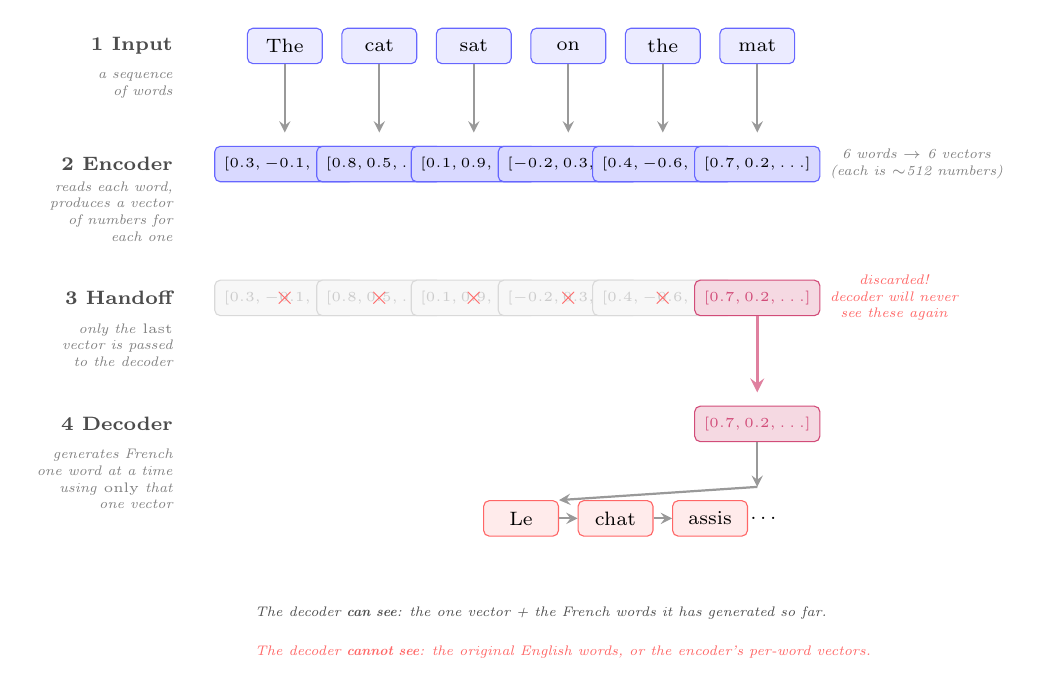
\begin{tikzpicture}[
    >=stealth,
    word/.style={rectangle, draw=blue!60, fill=blue!8, rounded corners=2pt,
                 minimum width=0.95cm, minimum height=0.45cm, font=\scriptsize},
    encout/.style={rectangle, draw=blue!60, fill=blue!15, rounded corners=2pt,
                   minimum width=0.95cm, minimum height=0.45cm, font=\tiny},
    vecbox/.style={rectangle, draw=purple!70, fill=purple!8, rounded corners=2pt,
                   minimum width=5.5cm, minimum height=0.7cm},
    vecnum/.style={font=\tiny\ttfamily, text=purple!70},
    outword/.style={rectangle, draw=red!60, fill=red!8, rounded corners=2pt,
                    minimum width=0.95cm, minimum height=0.45cm, font=\scriptsize},
    decbox/.style={rectangle, draw=red!50, fill=red!5, rounded corners=4pt,
                   minimum width=2.2cm, minimum height=1.2cm},
    steplabel/.style={font=\scriptsize\bfseries, text=black!70},
    note/.style={font=\tiny\itshape, text=black!50, align=center},
    noteleft/.style={font=\tiny\itshape, text=black!50, align=right, anchor=east},
    arr/.style={->, thick, black!40},
    bigarr/.style={->, very thick, purple!50},
    xmark/.style={font=\small\bfseries, text=red!60},
]
  % === ROW 1: Input sequence ===
  \node[steplabel, anchor=east] at (-0.8, 7) {\circled{1} Input};
  \node[noteleft] at (-0.8, 6.5) {a sequence\\of words};

  \node[word] (w1) at (0.5, 7) {The};
  \node[word] (w2) at (1.7, 7) {cat};
  \node[word] (w3) at (2.9, 7) {sat};
  \node[word] (w4) at (4.1, 7) {on};
  \node[word] (w5) at (5.3, 7) {the};
  \node[word] (w6) at (6.5, 7) {mat};

  % === ROW 2: Encoder produces per-word representations ===
  \node[steplabel, anchor=east] at (-0.8, 5.5) {\circled{2} Encoder};
  \node[noteleft] at (-0.8, 4.9) {reads each word,\\produces a vector\\of numbers for\\each one};

  \foreach \i/\x in {1/0.5, 2/1.7, 3/2.9, 4/4.1, 5/5.3, 6/6.5} {
    \draw[arr] (w\i.south) -- (\x, 5.9);
  }

  \node[encout] (e1) at (0.5, 5.5) {\tiny$[0.3, \text{-}0.1, \ldots]$};
  \node[encout] (e2) at (1.7, 5.5) {\tiny$[0.8, 0.5, \ldots]$};
  \node[encout] (e3) at (2.9, 5.5) {\tiny$[0.1, 0.9, \ldots]$};
  \node[encout] (e4) at (4.1, 5.5) {\tiny$[\text{-}0.2, 0.3, \ldots]$};
  \node[encout] (e5) at (5.3, 5.5) {\tiny$[0.4, \text{-}0.6, \ldots]$};
  \node[encout] (e6) at (6.5, 5.5) {\tiny$[0.7, 0.2, \ldots]$};

  \node[note, anchor=west] at (7.3, 5.5) {6 words $\to$ 6 vectors\\(each is $\sim$512 numbers)};

  % === ROW 3: The bottleneck — only LAST vector passed ===
  \node[steplabel, anchor=east] at (-0.8, 3.8) {\circled{3} Handoff};
  \node[noteleft] at (-0.8, 3.2) {only the \emph{last}\\vector is passed\\to the decoder};

  % Grey out first 5
  \node[encout, draw=black!15, fill=black!3, text=black!20] (g1) at (0.5, 3.8) {\tiny$[0.3, \text{-}0.1, \ldots]$};
  \node[encout, draw=black!15, fill=black!3, text=black!20] (g2) at (1.7, 3.8) {\tiny$[0.8, 0.5, \ldots]$};
  \node[encout, draw=black!15, fill=black!3, text=black!20] (g3) at (2.9, 3.8) {\tiny$[0.1, 0.9, \ldots]$};
  \node[encout, draw=black!15, fill=black!3, text=black!20] (g4) at (4.1, 3.8) {\tiny$[\text{-}0.2, 0.3, \ldots]$};
  \node[encout, draw=black!15, fill=black!3, text=black!20] (g5) at (5.3, 3.8) {\tiny$[0.4, \text{-}0.6, \ldots]$};

  % Highlight last one
  \node[encout, draw=purple!70, fill=purple!15, text=purple!70] (glast) at (6.5, 3.8) {\tiny$[0.7, 0.2, \ldots]$};

  % X marks on discarded ones
  \node[xmark] at (0.5, 3.8) {$\times$};
  \node[xmark] at (1.7, 3.8) {$\times$};
  \node[xmark] at (2.9, 3.8) {$\times$};
  \node[xmark] at (4.1, 3.8) {$\times$};
  \node[xmark] at (5.3, 3.8) {$\times$};

  \node[note, anchor=west, text=red!60] at (7.3, 3.8) {discarded!\\decoder will never\\see these again};

  % Arrow down from last vector
  \draw[bigarr] (glast.south) -- (6.5, 2.6);

  % === ROW 4: Decoder generates output ===
  \node[steplabel, anchor=east] at (-0.8, 2.2) {\circled{4} Decoder};
  \node[noteleft] at (-0.8, 1.5) {generates French\\one word at a time\\using \emph{only} that\\one vector};

  % The single vector the decoder has
  \node[encout, draw=purple!70, fill=purple!15, text=purple!70] (dvec) at (6.5, 2.2) {\tiny$[0.7, 0.2, \ldots]$};

  % Decoder generates words
  \draw[arr] (dvec.south) -- (6.5, 1.4);
  \node[outword] (o1) at (3.5, 1.0) {Le};
  \node[outword] (o2) at (4.7, 1.0) {chat};
  \node[outword] (o3) at (5.9, 1.0) {assis};
  \node[font=\scriptsize] at (6.6, 1.0) {\ldots};

  \draw[arr] (6.5, 1.4) -- (o1.north east);
  \draw[arr] (o1.east) -- (o2.west);
  \draw[arr] (o2.east) -- (o3.west);

  % What the decoder CAN and CANNOT see
  \node[note, align=left, text=black!70, anchor=north west] at (0, 0.0)
    {The decoder \textbf{can see}: the one vector + the French words it has generated so far.};
  \node[note, align=left, text=red!60, anchor=north west] at (0, -0.5)
    {The decoder \textbf{cannot see}: the original English words, or the encoder's per-word vectors.};

  % circled number helper
\end{tikzpicture}
\caption{Without attention: the full pipeline. \circled{1}~The input is a sequence of English words. \circled{2}~The encoder processes each word and produces a vector of numbers for each. \circled{3}~But only the \emph{last} vector is handed to the decoder --- the others are discarded. \circled{4}~The decoder must generate the entire French sentence from that one vector, plus the French words it has already produced. It cannot go back and look at the English.}
\end{figure}

\textbf{Attention} was the fix.

The idea, introduced by Bahdanau et al.\ in 2014 \cite{bahdanau2014neural}, was: what if the decoder, instead of working from a single compressed summary, could \emph{look back} at the encoder's representation of every single input word, and decide which ones are relevant right now?

So when the decoder is about to produce the French word for ``cat,'' it can attend strongly to the English word ``cat'' in the input and mostly ignore everything else.
When it is producing a verb, it can attend to the corresponding verb in the source.
Each output word gets to choose its own context.

\begin{figure}[htb]
\centering
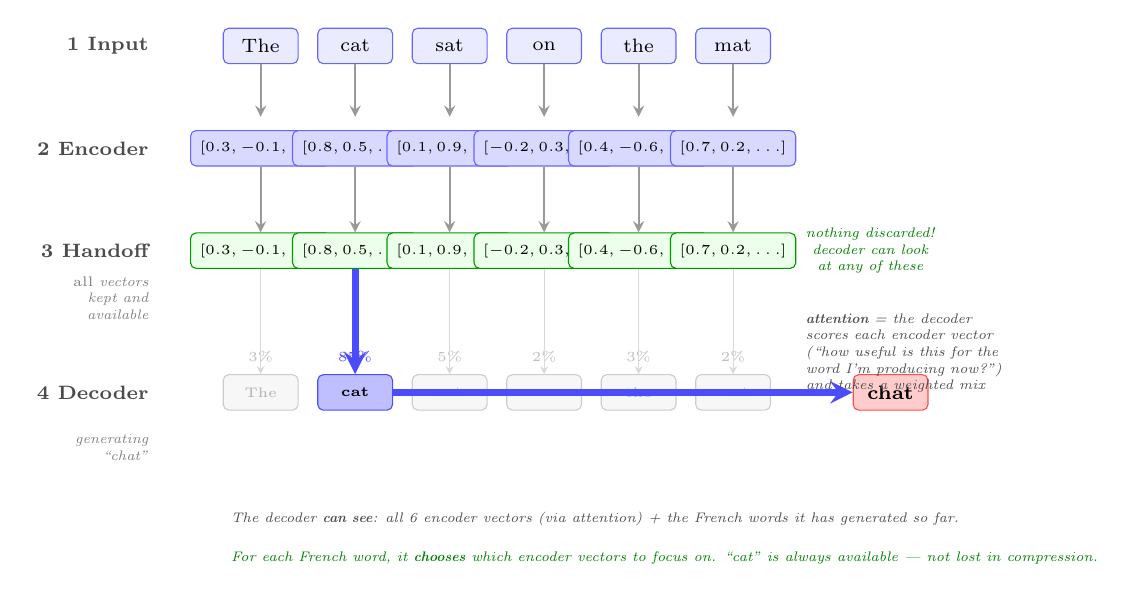
\begin{tikzpicture}[
    >=stealth,
    word/.style={rectangle, draw=blue!60, fill=blue!8, rounded corners=2pt,
                 minimum width=0.95cm, minimum height=0.45cm, font=\scriptsize},
    encout/.style={rectangle, draw=blue!60, fill=blue!15, rounded corners=2pt,
                   minimum width=0.95cm, minimum height=0.45cm, font=\tiny},
    kept/.style={rectangle, draw=green!60!black, fill=green!8, rounded corners=2pt,
                 minimum width=0.95cm, minimum height=0.45cm, font=\tiny},
    outword/.style={rectangle, draw=red!60, fill=red!8, rounded corners=2pt,
                    minimum width=0.95cm, minimum height=0.45cm, font=\scriptsize},
    highlight/.style={rectangle, draw=blue!70, fill=blue!25, rounded corners=2pt,
                      minimum width=0.95cm, minimum height=0.45cm, font=\tiny\bfseries},
    dim/.style={rectangle, draw=black!20, fill=black!3, rounded corners=2pt,
                minimum width=0.95cm, minimum height=0.45cm, font=\tiny, text=black!30},
    generating/.style={rectangle, draw=red!70, fill=red!20, rounded corners=2pt,
                       minimum width=0.95cm, minimum height=0.45cm, font=\scriptsize\bfseries},
    steplabel/.style={font=\scriptsize\bfseries, text=black!70},
    note/.style={font=\tiny\itshape, text=black!50, align=center},
    noteleft/.style={font=\tiny\itshape, text=black!50, align=right, anchor=east},
    arr/.style={->, thick, black!40},
    strong/.style={->, line width=2.5pt, blue!70},
    weak/.style={->, line width=0.3pt, black!15},
]
  % === ROW 1: Input sequence (same as before) ===
  \node[steplabel, anchor=east] at (-0.8, 8.5) {\circled{1} Input};

  \node[word] (w1) at (0.5, 8.5) {The};
  \node[word] (w2) at (1.7, 8.5) {cat};
  \node[word] (w3) at (2.9, 8.5) {sat};
  \node[word] (w4) at (4.1, 8.5) {on};
  \node[word] (w5) at (5.3, 8.5) {the};
  \node[word] (w6) at (6.5, 8.5) {mat};

  % === ROW 2: Encoder (same as before) ===
  \node[steplabel, anchor=east] at (-0.8, 7.2) {\circled{2} Encoder};

  \foreach \i/\x in {1/0.5, 2/1.7, 3/2.9, 4/4.1, 5/5.3, 6/6.5} {
    \draw[arr] (w\i.south) -- (\x, 7.6);
  }

  \node[encout] (e1) at (0.5, 7.2) {\tiny$[0.3, \text{-}0.1, \ldots]$};
  \node[encout] (e2) at (1.7, 7.2) {\tiny$[0.8, 0.5, \ldots]$};
  \node[encout] (e3) at (2.9, 7.2) {\tiny$[0.1, 0.9, \ldots]$};
  \node[encout] (e4) at (4.1, 7.2) {\tiny$[\text{-}0.2, 0.3, \ldots]$};
  \node[encout] (e5) at (5.3, 7.2) {\tiny$[0.4, \text{-}0.6, \ldots]$};
  \node[encout] (e6) at (6.5, 7.2) {\tiny$[0.7, 0.2, \ldots]$};

  % === ROW 3: Handoff — ALL vectors kept ===
  \node[steplabel, anchor=east] at (-0.8, 5.9) {\circled{3} Handoff};
  \node[noteleft] at (-0.8, 5.3) {\emph{all} vectors\\kept and\\available};

  \node[kept] (k1) at (0.5, 5.9) {\tiny$[0.3, \text{-}0.1, \ldots]$};
  \node[kept] (k2) at (1.7, 5.9) {\tiny$[0.8, 0.5, \ldots]$};
  \node[kept] (k3) at (2.9, 5.9) {\tiny$[0.1, 0.9, \ldots]$};
  \node[kept] (k4) at (4.1, 5.9) {\tiny$[\text{-}0.2, 0.3, \ldots]$};
  \node[kept] (k5) at (5.3, 5.9) {\tiny$[0.4, \text{-}0.6, \ldots]$};
  \node[kept] (k6) at (6.5, 5.9) {\tiny$[0.7, 0.2, \ldots]$};

  \foreach \i/\x in {1/0.5, 2/1.7, 3/2.9, 4/4.1, 5/5.3, 6/6.5} {
    \draw[arr] (e\i.south) -- (k\i.north);
  }

  \node[note, anchor=west, text=green!50!black] at (7.3, 5.9) {nothing discarded!\\decoder can look\\at any of these};

  % === ROW 4: Decoder step — generating "chat" ===
  \node[steplabel, anchor=east] at (-0.8, 4.1) {\circled{4} Decoder};
  \node[noteleft] at (-0.8, 3.4) {generating\\``chat''};

  % Show the kept vectors again, but dimmed/highlighted based on attention
  \node[dim] (a1) at (0.5, 4.1) {\tiny The};
  \node[highlight] (a2) at (1.7, 4.1) {\tiny cat};
  \node[dim] (a3) at (2.9, 4.1) {\tiny sat};
  \node[dim] (a4) at (4.1, 4.1) {\tiny on};
  \node[dim] (a5) at (5.3, 4.1) {\tiny the};
  \node[dim] (a6) at (6.5, 4.1) {\tiny mat};

  % Attention weights
  \node[font=\tiny, text=black!25] at (0.5, 4.55) {3\%};
  \node[font=\tiny, text=blue!70] at (1.7, 4.55) {85\%};
  \node[font=\tiny, text=black!25] at (2.9, 4.55) {5\%};
  \node[font=\tiny, text=black!25] at (4.1, 4.55) {2\%};
  \node[font=\tiny, text=black!25] at (5.3, 4.55) {3\%};
  \node[font=\tiny, text=black!25] at (6.5, 4.55) {2\%};

  % Arrows from kept vectors to attention row
  \draw[weak] (k1.south) -- (a1.north);
  \draw[strong] (k2.south) -- (a2.north);
  \draw[weak] (k3.south) -- (a3.north);
  \draw[weak] (k4.south) -- (a4.north);
  \draw[weak] (k5.south) -- (a5.north);
  \draw[weak] (k6.south) -- (a6.north);

  % Output word
  \node[generating] (out) at (8.5, 4.1) {chat};
  \draw[strong] (a2.east) -- (out.west);

  % Annotation: what attention IS
  \node[note, anchor=west, text=black!70, align=left] at (7.3, 4.6)
    {\textbf{attention} = the decoder\\scores each encoder vector\\(``how useful is this for the\\word I'm producing now?'')\\and takes a weighted mix};

  % === ROW 5: What the decoder can see ===
  \node[note, align=left, text=black!70, anchor=north west] at (0, 2.7)
    {The decoder \textbf{can see}: all 6 encoder vectors (via attention) + the French words it has generated so far.};
  \node[note, align=left, text=green!50!black, anchor=north west] at (0, 2.2)
    {For each French word, it \textbf{chooses} which encoder vectors to focus on. ``cat'' is always available --- not lost in compression.};

\end{tikzpicture}
\caption{With attention: the full pipeline. \circled{1}~Same input. \circled{2}~Same encoder --- a vector for each word. \circled{3}~But now \emph{all} vectors are kept and handed to the decoder. \circled{4}~When generating ``chat,'' the decoder scores every encoder vector --- ``how relevant is `cat' right now? how relevant is `mat'?'' --- and takes a weighted combination. 85\% of its context comes from the vector for ``cat.'' The next word will re-score and pick a different focus. That scoring process is what \emph{attention} means.}
\end{figure}

This was a huge deal.
It was not a new model --- it was an add-on to existing RNN encoder-decoders.
But it dramatically improved translation quality, especially for long sentences, because the decoder no longer had to rely on a single bottleneck vector.

The key word in the abstract is \emph{also}: ``The best performing models \textbf{also} connect the encoder and decoder through an attention mechanism.''
The architecture was still RNN-based.
Attention was a supplement, not a replacement.
The recurrence was still there.
The sequential processing was still there.
The parallelism problem was still there.

Attention was clearly a good idea.
The question that the eight authors of this paper asked was: what if attention was not just a good idea, but the \emph{only} idea you needed?
